\documentclass[%
 reprint,
%superscriptaddress,
%groupedaddress,
%unsortedaddress,
%runinaddress,
%frontmatterverbose, 
%preprint,
%showpacs,preprintnumbers,
%nofootinbib,
%nobibnotes,
%bibnotes,
 amsmath,amssymb,
 aps,
%pra,
%prb,
%rmp,
%prstab,
%prstper,
%floatfix,
]{revtex4-1}

\usepackage{graphicx}   % for figures
\usepackage{epstopdf}
%\usepackage{epsfig}
%draft
\usepackage{dcolumn}
\usepackage{bm}	
\usepackage{amsmath}			
\usepackage{amsfonts}			
\usepackage{amssymb}			
\usepackage{latexsym}			
%\usepackage{floatrow}
\usepackage{color}
%\usepackage{thumbpdf}

\begin{document}

\title{Accounting for speckle-scale beam-bending in classical ray tracing schemes}
\author{C. Ruyer}\email{charles.ruyer@cea.fr}
\author{A. Debayle}
\author{P. Loiseau}
\author{M. Casanova}
\author{P. E. Masson-Laborde}
\affiliation{CEA, DAM, DIF, F-91297 Arpajon, France}

\begin{abstract}
The advection by a flow of ponderomotively  driven density fluctuations may lead to the deflection of a laser pulse. This effect,  also called beam bending, may modify the irradiation geometry and energy deposition in high energy laser plasma experiments. A kinetic modeling of beam-bending of a small Gaussian laser pulse is proposed and validated by mean of "particle-in-cell" simulations over a vast parametric domain, demonstrating the importance of capturing correctly the kinetic damping of ion-acoustic waves. This simple modeling is further extended to spatially smoothed laser beam to describe the speckle scale beam-bending. A Monte-Carlo method is proposed to include this model on classical ray tracing schemes. A quantitative comparison with large scale "particle-in-cell" simulations is successfully carried. 
\end{abstract}

\maketitle

\section{Introduction}
The study of many astrophysical phenomenon \cite{Drake_2012}, High-energy-density physics \cite{Drake2006}, and inertial confinement fusion \cite{Lindl_2004,He_2007,Cavailler_2005} are performed using multi-kilojoule laser pulses interaction with plasmas. With such beams, the matter can be heated to millions of degrees with Mega to Gigabar pressure, hence providing unique plasma conditions on earth. Quantitative understanding of 
multi-kilojoule laser pulse propagation through plasma is mandatory to correctly interpret all these experiments. In particular, a great effort has been dedicated to understand the mechanisms responsible of the plasma heating,  and  predicting various instabilities that may arise during the laser pulse propagation such as stimulated Raman or Brillouin scattering  \cite{Shen_1965,Forslund_1973,POP_Liu_2009,hao_2013}, cross-beam energy transfer \cite{hao_2016}, two-plasmon decay  \cite{Dubois_1995,Russell_2001} or self-focusing  \cite{Wagner_1968}.

In most experiments involving  nanosecond-long pulses, optical smoothing techniques  such as the Random-Phase-Plates (RPP) and the smoothing by spectral dispersion (SSD), are often used in order to reach a satisfactorily control of the laser intensity profile \cite{Kato_1984}.
These techniques, which usually  consist in degrading the spatial (RPP) and temporal coherence (SSD) of the electromagnetic wave,  result in a diffraction pattern  with intensity fluctuations on the scale of a few wavelength : the so-called speckles. 
Different experimental and theoretical studies unravelled the non-negligible impact of these micron-scale intensity fluctuations on macroscopic quantities such as the energy deposition region  \cite[]{POP_Delamater_1996,Huser_2009}, the scattering direction  of the light wave \cite{Epstein_1986,PRL_Moody_96,POP_Debayle_2018,POP_Duluc_2019,Yin_2019,POP_Huller_2020} or the amount of expected reflectivity \cite[]{POP_Laffite_2010,PRL_Rousseaux_2016,POP_Masson_2016,Glize_2017,Winjum_2019}.
It is therefore of critical importance in our modeling of laser-plasma interaction experiments to capture the diffraction pattern and the associated hot-spot fluctuations. 
However, reconciling the light-wave micron or sub-micron wavelength and  femtosecond temporal period with many experimental  hydrodynamical scales  (millimeters and nanoseconds) is extremely challenging in a self-consistent numerical manner. 

%More generally, a mojor issue of  laser-plasma interaction relevant for NIF-class facilities lies in the need of a better description of the light propagation in a large scale plasma, without resorting to a fine discretisation of the laser-wavelength that would  be prohibitive for modeling hydrodynamics scale experiments.
Regarding the nanosecond and millimeter scales of interest here, a hydrodynamical description of the plasma can be coupled with Maxwell equations \cite{Berger_1995,Still_2006,Loiseau_2006, Huller_2006}, however these  formalisms may appear to be  too heavy numerically whenever  multi-dimensional effects,  solid-density physics or radiative phenomenons arise.

In such systems, we usually resort to a rough description of light \cite[]{POP_Zhang_2014,Lefebvre_2018},  such as the classical ray tracing scheme which, in its native form, only captures the wave refraction and basic energy deposition.
The proper description, by the ray tracing scheme,  of simple  light quantities  such as the intensity  of the wave or its local spectrum, is still an active area of research  \cite{Egorchenkov_2001, Colaitis_2014, Strozzi_2017}.
Although a large effort is made in improving these schemes by including back or side scattering of the light caused by wave mixing processes \cite[]{Strozzi_2017,POP_Debayle_2019},  
modeling the impact of plasma smoothing effects on the pulse propagation properties remains vastly unexplored \cite[]{POF_Anderson,POP_Still_2000,POP_Grech_2006,PRL_Grech_2009}.
More specifically, we address in this paper the beam bending  of  a laser pulse, as studied in Refs. \cite{PRL_Hinkel_1996,POP_Rose_96,Vu_1997,POP_Rose_97,PRL_Montgomery} and which occurs when the ponderomotively driven density hole  during the propagation of a laser pulse is advected by the flow. It results,  due to a wave-guide effect, to the deflection of the electromagnetic wave off its original propagating axe. It is important to note that  this effect may take place in a perfectly homogeneous plasma and thus adds up to the usual refraction of light caused by density gradients. 
We will first introduce an analytical model predicting the deflection angle, in both the asymptotic and transient regime, of a Gaussian laser pulse including the kinetic damping of acoustic waves and validated by  a large number of  Particle-in-cell (PIC) simulations. 
Proof will then be made that the kinetic  physics of  driven ion acoustic wave damping, essential to obtain accurate predictions, can be   included as a correction in the 
 the calculation of the ponderomotive force of interest for capturing the beam bending rates in fluid-based codes such as HERA or PF3D  \cite{Berger_1995,Still_2006,Loiseau_2006, Huller_2006}. 
Our analytical  model  will then be extended to
the ray-tracing description of the propagation of an energetic RPP-beam (without temporal smoothing), by
combining the single-speckle scattering angle with a Monte Carlo modeling of the speckles distribution in vacuum. 
A validation of our  predictions with both large scale PIC simulations and a paraxial and ponderomotively-corrected fluid codes will be carried,
%The effect of temporal smoothing techniques on the bending dynamics will then be discussed, modeled and validated with large scale PIC simulations,
followed by our concluding remarks and perspectives. Finally, the SI unit system is used and 2D Cartesian geometry only will be considered throughout this publication. 

\section{Beam bending of a Gaussian laser pulse}\label{sec:gauss}
\subsection{Asymptotic regime theory}
For simplicity, we will assume subsequently  that the electromagnetic waves are forward propagating only, thus excluding any back-scattering. 
Reference \cite{POP_Rose_96} models the beam bending in the hydrodynamical framework. Evidence is made that the ponderomotive driven acoustic perturbations, deformed and advected by the  flow, may significantly deflects the electromagnetic wave off its course. We address here the asymptotic limit eventually reached by a Gaussian pulse propagating in a flowing plasma, the transient regime will be discussed subsequently.

Let introduce,$ \langle X\rangle_{k_y} $ and  $ \langle X\rangle_y $, the  average of $ X $ in the Fourier and the real space respectively, defined as
\begin{align}
\langle X \rangle_{k_y} &= \frac{\int X(k_y) \vert E(k_y,x,t) \vert^2 dk_y }{\int   \vert E(k_y,x,t) \vert^2 dk_y}\, , \label{eq:kmoy}\\
\langle X \rangle_{y}&= \frac{\int X(y)\vert E(y,x,t) \vert^2 dy }{\int   \vert E(y,x,t) \vert^2 dy}\, , \label{eq:ymoy}
\end{align}
where $ E(k_y,x,t) $ is the transverse Fourier transform of the electric field, Eqs. (24) and (26) of Ref.  \cite{POP_Rose_96} relates the  spatial evolution of $ \langle \bf{k}\rangle$ to  $\delta n(x,y,t)$, $ n_0$ and $n_c$ (the perturbed, averaged and critical electron density respectively) through 
\begin{align}
 \frac{1}{k_0}\frac{d \langle k_y\rangle_{k}    }{d x}& =- \frac{1  }{2} \frac{n_0 }{n_c}   \left \langle \frac{\partial_y \delta n }{n_0}  \right  \rangle_y   \, ,\label{eq:rose26}\\
  \frac{d \langle y\rangle_{y}    }{d x} &= \frac{ \langle k_y\rangle_{k}  }{k_0} \, ,\label{eq:rose24}
\end{align}
where $k_0$ is the laser wave vector in vacuum.

The right-hand side of the Eq. \eqref{eq:rose26} vanishes when the density profile remain an even function of the transverse position $y$. In order to assess the influence of a flow on the ponderomotive density fluctuations, we will first introduce the perturbed velocity $v = v_d +\delta v$ and  make use of the conservation of density and momentum. To leading order in $\delta v$ and $\delta n$ and neglecting all longitudinal ($x$) spatial derivatives, we obtain 
\begin{align}
(\partial_t + v_d  \cdot \partial_y) \frac{  \delta n }{n_0} &= - \partial_y\delta v \, ,\label{eq:hydro1} \\
(\partial_t + v_d  \cdot \partial_y) \delta v + 2\nu \delta v  &= - c_s^2\partial_y^2\left(\frac{  \delta n }{n_0} +  \Phi  \right) \, ,\label{eq:hydro2} 
\end{align}
where $ \Phi = I /(4v_g n_c T_e )$ is the normalized laser ponderomotive potential,  $c_s$, $v_g$ and $I$  are the plasma sound speed, laser group velocity and intensity respectively.
The damping term, $\nu$, of Eq. \eqref{eq:hydro2} accounts for the ion acoustic wave damping mainly due to the Landau phase mixing process. The self-consistent description of this kinetic effect in the hydrodynamic equations remains a challenging problem. Different works suggest a fluid closure at order 3 or 4 is necessary to recover some kinetic behavior of the dispersion relation~\cite{PRL_Hammett_1990,POF_Chang_1992}. Yet, to simplify our analysis, we introduce empirically this friction term to describe the ion acoustic wave damping.
 Combining Eqs. \eqref{eq:hydro1} and \eqref{eq:hydro2} gives 
\begin{align}
 \{ (c_s^2-v_d^2)\partial_y^2 -\partial_t \partial_t\}    \frac{  \delta n }{n_0} - 2 v_d \partial_y  \partial_t \frac{  \delta n }{n_0}   \nonumber \\
-2\nu  (\partial_t + v_d  \cdot \partial_y) \frac{  \delta n }{n_0}   = - c_s^2\partial_y^2 \Phi  \, .\label{eq:hydro3} 
\end{align}
The asymptotic limit ($\partial_t\equiv 0$) yields 
\begin{align}
 (c_s^2-v_d^2)\partial_y^2    \frac{  \delta n }{n_0}  
-2\nu    v_d  \cdot \partial_y \frac{  \delta n }{n_0}   = - c_s^2\partial_y^2 \Phi  \, , \label{eq:hydro3b} 
\end{align}
showing that the density perturbation does not coincide with the ponderomotive potential when $\nu    v_d $ is not vanishing.
In that context, Ref. \cite{POP_Rose_96,POP_Rose_97} showed that the beam bending rate in the fluid framework reads:
\begin{equation}
\frac{1}{k_0}\frac{d \langle k_y\rangle_{k}    }{d x} = \frac{K_\mathrm{rad} }{\sigma} \frac{n_0 }{n_c}  \frac{  I(k_y) }{ 2 v_g n_c T_e }  f(M_0,\gamma_0)\, ,\label{eq:dthetarose26}
\end{equation}
where $K_\mathrm{rad} \simeq 1.36$  and 
\begin{equation}
 f(M,\gamma) =\frac{2 }{\pi }  \int_0^{\pi/2}\frac{ M \gamma \cos(\theta)^2  d\theta}{(1-M \cos(\theta)^2)^2 +4M^2 \gamma^2 \cos(\theta)^2}  \, .\label{eq:frose26}
\end{equation}
These predictions use the Landau ion acoustic damping rate in the free wave regime, i.e. assuming that the ponderomotively driven density perturbation propagates at the sound speed.

However, in the asymptotic limit of interest here, \emph{i.e.} for a stationary laser beam, the density perturbation propagates, in the rest-frame of the plasma, at a velocity $-v_d\ne -c_s$ owing to the advection by the flow. Therefore, the usual  free-mode perturbation model fails to capture the adequate damping rate. However, the kinetic response of an acoustic-like perturbation to a ponderomotive potential has been derived in Ref.  \cite{POF_Drake_1973}  [Eq. (12)] for a Maxwellian plasma.
Note that unlike Ref. \cite{POF_Drake_1973}, we use the convention $E=E_0\cos(k_0x-w_0t)$ (where $\omega_0$ is the laser frequency).
Introducing the wave vector component $k_y$ transverse to the $x$-aligned laser propagating direction,  the density perturbation verifies and its magnitude $\vert k_y\vert$, 
\begin{align}
 \frac{ \delta n (k_y) }{n_0}  &=   \frac{  I(k_y) }{ 8 v_g n_c T_e }  \mathcal{Z}'( \xi_e)   \frac{ 1- \frac{ \mathcal{Z}'( \xi_i)  }{ k_y^2\lambda_{Di}^2  }   }{  1- \frac{ \mathcal{Z}'( \xi_i)  }{ k_y^2\lambda_{Di}^2  }- \frac{ \mathcal{Z}'( \xi_e)  }{ k_y^2\lambda_{De}^2  } }    \, , \label{eq:drake}\\
\xi_{e/i } &= \frac{   \omega- k_y v_d }{ 2^{1/2}  \vert k_y\vert }  \sqrt{ \frac{ m_{e/i } }{ T_{e/i }}  }  \label{eq:xiie}   \,  ,
\end{align}
We introduced $ \mathcal{Z}$, the plasma dispersion function \cite{Fried_Gell-Mann_1960} and its arguments $\xi_{e } $ and $\xi_{i }$, both proportional to the $\omega/\vert k_y \vert$. 
Hence, in our case, we may use $\omega=k_yv_d$ in Eq. \eqref{eq:xiie} which gives 
\begin{align}
\xi_{e } &=\frac{   M_0 }{ 2^{1/2} }  \frac{k_y}{\vert k \vert }\sqrt{ \frac{ Z m_{e } }{ m_i }  } \sqrt{1+ \frac{\gamma_i T_i }{ ZT_e }  }   \, , \\
\xi_{i } &= \frac{   M_0}{ 2^{1/2} }  \frac{k_y}{\vert k \vert }\sqrt{ \frac{Z T_{e } }{ T_{i }} +\gamma_i  }    \, ,
\end{align}
with $c_s=[(ZT_e+\gamma_i T_i)/m_i]^{1/2}$ and $\gamma_i$ the ion adiabatic index.
Note that the self-consistent description of plasmas in PIC codes does not require any  fluid closure, hence the sound speed value is set by the kinetic dispersion relations  rather than a presumed  equation of states and thus do not necessarily co\"incide with the above relations. 
Throughout this study, use will be made of  $\gamma_i=3$ for fluid simulations, as in most fluid-based laser-plasma interaction studies, although a difference is to be expected  regarding PIC simulation. The exact kinetic calculation of $\gamma_i$ is left for future work.

As the length scale of the density fluctuations verify  $k\lambda_{Di} \ll 1 $, Eq.  \eqref{eq:drake} can be simplified to 
 \begin{align}
 \frac{ \delta n(k_y) }{n_0}  &=   \frac{ - I(k_y) }{ 4 v_g n_c T_e }  \alpha_ \mathrm{kin}    \, , \nonumber \\
 \alpha_ \mathrm{kin}    & = \frac{-\mathcal{Z}'( \xi_e) }{2}\frac{\mathcal{Z}'( \xi_i)   }{  \mathcal{Z}'( \xi_i) +\mathcal{Z}'( \xi_e)\frac{ T_i }{  ZT_e} } \, , \label{eq:drakef} 
\end{align}
with  $\alpha_ \mathrm{kin}    =1$  when $v_d=0$. 

We may now evaluate the right-hand side of Eq. \eqref{eq:rose26} in real space, which, after an inverse Fourier transform and a derivation of Eq. \eqref{eq:drakef}, reads
\begin{align}
 \left \langle\partial_y  \left( \frac{ \delta n }{n_0} \right)  \right  \rangle_y&=     \left \langle\int \frac{dk}{2\pi}   e^{ik y} i k  \frac{ -I(k) \alpha_ \mathrm{kin}  }{ 4 v_g n_c T_e }    \right  \rangle_y \, . \label{eq:1}
\end{align}
For a spatially Gaussian pulse defined as $I(y)=I_0g(y)$ with  $ g(y) = \exp(-2y^2/\sigma^2)$, we have $I(k_y)=I_0\sigma \sqrt{\pi/2}  \exp(-k_y^2\sigma^2/8)$ and  $\left \langle \exp(ik_y y) \right  \rangle_y= \exp(-k_y^2\sigma^2/8)$. We thus obtain
\begin{align}
  \left \langle\partial_y  \left( \frac{ \delta n }{n_0} \right)  \right  \rangle_y&=   
  \frac{ -I_0  }{ 4 v_g n_c T_e } \frac{\sigma }{ 2 }\int \frac{dk}{\sqrt{2\pi}} e^{-k^2\sigma^2/4}   i k    \alpha_ \mathrm{kin}   \, . \label{eq:2}
 \end{align}
 For the following, it is essential to notice that  the real and imaginary part of  $\alpha_ \mathrm{kin}(k_yv_d/\vert k_y\vert)$ are even and odd functions of $k_y$ respectively.
 Hence,  using $\int dk_y\vert k_y\vert \exp(-k_y^2\sigma^2/4)=4/\sigma^2$, 
 \begin{align} 
 \left \langle\partial_y  \left( \frac{ \delta n }{n_0} \right)  \right  \rangle_y&=   
  \frac{ I_0  }{ 2 v_g n_c T_e } \sqrt{\frac{\pi}{2}}\frac{\alpha_{\mathrm{kin},i} }{ \sigma }   \, , \label{eq:3}\\
\alpha_{\mathrm{kin},i} &= \Im\left[\alpha_\mathrm{kin}\left(\frac{k_yv_d}{\vert k_y\vert}\right)\right] \frac{k_y}{\vert k_y\vert} \, , \nonumber
\end{align}
where $\Im$ is the imaginary part of a complex and $\alpha_{\mathrm{kin},i} $, defined as above, is independent of $k_y$. 

Combined with Eq. \eqref{eq:rose26}, we obtain the final beam bending rate
  \begin{align}
\frac{1}{k_0} \frac{d \langle k_y\rangle_{k}    }{d x}& = - \frac{n_0 }{n_c}  \frac{  I_0 }{ 4 v_g n_c T_e } \sqrt{\frac{2}{\pi}}   \frac{\alpha_{\mathrm{kin},i} }{ \sigma}     
  \, ,\label{eq:bbf}
\end{align}

We will now derive, from Eqs. \eqref{eq:rose24} and \eqref{eq:bbf}, the displacement and deflection angle of a Gaussian beam in a homogeneous plasma.
We will assume that the beam focal plane lies in $x=x_\mathrm{foc}$, the plasma extend from $\Delta x \equiv x-x_\mathrm{foc}=-L_x/2$ to $x=L_x/2$, is infinite in the $y$ direction and characterized by an ion/electron mass, density and temperature given by $m_{i/e}$, $Zn_i=n_e$ and $T_{i,e}$, respectively.
Replacing $I_0$ by $ I_0/(1+\Delta x^2/z_c^2)$ and $\sigma$ by $ \sigma\sqrt{1+\Delta x^2/z_c^2}$  (where $z_c=\pi f^2\lambda_0$ is the Rayleigh length) in Eq. \eqref{eq:bbf}  to account for the slowly varying ($z_c\gg \sigma$) longitudinal intensity profile and integrating it from $x=-L_x/2$ to $L_x/2$, we obtain the following asymptotic deflection angle in the small angle limit ($\Delta \theta^{\infty} \ll 1$)
  \begin{align}
\Delta \theta^{\infty} & =\frac{n_0 }{n_c}  \frac{  I_0   \alpha_{\mathrm{kin},i}}{ 4 v_g n_c T_e } \sqrt{\frac{2}{\pi}}      \frac{z_c}{\sigma} \frac{L_x}{z_c} \left[ 1+\left(\frac{L_x}{2z_c}\right)^2\right]^{-1/2}
  \, .\label{eq:dth}
\end{align}
Likewise the centro\"id displacement at $x = L_x$ verifies
 \begin{align}
\Delta y^{\infty} & = \frac{n_0 }{n_c}  \frac{  I_0   \alpha_{\mathrm{kin},i}}{ 4 v_g n_c T_e } \sqrt{\frac{2}{\pi}}     \frac{L_x}{2z_c} \left[ 1+\left(\frac{L_x}{2z_c}\right)^2\right]^{-1/2} L_x
  \, .\label{eq:dy}
\end{align}

Hence, the average wave vector deflection for a speckle modeled by a Gaussian pulse of length $L_x=2z_c $ reads: 
 \begin{align}
\Delta \theta^{\infty}(L_x=2z_c) & = \frac{n_0 }{n_c}  \frac{  I_0   \alpha_{\mathrm{kin},i}}{ 2 v_g n_c T_e } \sqrt{\frac{1}{\pi}}      \frac{z_c}{\sigma}   
  \, .\label{eq:dthf}
\end{align}

\subsection{Comparison with PIC simulations}
In order to validate our results, we performed Smilei \cite[]{Smilei} PIC simulations  of a Gaussian laser pulse crossing a fully ionized carbon plasma drifting along the direction transverse to the laser propagation axis. 
Subsequently, all PIC quantities are given for a $\lambda_0=1\,\rm\mu m$ laser wavelength.
The 2D simulation size is $L_x \times L_y = 128 \times 128\, \rm \mu$m$^2$ with fully periodic boundary  conditions in the $y$ direction, and absorbant (Silver-M\"uller) for the field and for the particles in the $x$ direction.
A Gaussian laser pulse propagating in the $+x$ direction was injected from the left boundary with the spatial profile at best focus $E_0\exp(-y^2/\sigma^2)$ with $\sigma=f\lambda_0$, focused in the center of the simulation domain with a focal number $f = 5$ and flat temporal envelope preceded by a 1 ps linear rise. 
A fourth order interpolation scheme is used with 36 particles per mesh per species, 20 points per laser wavelength and 14 points per laser temporal period. The plasma density is constant everywhere except on 14 microns close to both $\pm x$ boundaries so that the effective plasma length is 100 microns.

In order to isolate the beam bending as much as possible in our simulations, choice has been made to use $T_i=ZT_e$ for reducing the stimulated Brillouin backward scattering. The electron density is fixed to $n_e =0.1n_c $ with a $y$-aligned drift velocity, $v_y=v_d$, for both the electron and ion populations.
To validate the beam bending rate in a regime where PIC simulations are not numerically too constraining, we selected two sets of plasma parameters $(T_e, T_i )= (500\, $eV$, 3\, $keV$)$ and $(T_e, T_i )= (5\, $keV$, 30 \,$keV$)$. Finally, the maximum laser intensity used are either $I_0 = 10^{16} \,\rm W.cm^2$ or $I_0 = 3 \times10^{15} \,\rm W.cm^2$ for the case  $T_e=5\, \rm keV$  and $I_0 = 10^{15} \,\rm W.cm^2$ $I_0 = 3 \times10^{14} \,\rm W.cm^2$ for the case $T_e=500\, \rm eV$, thus corresponding to $\delta n_0/n_0=0.031$ or $0.1$, respectively.

\begin{figure}
\begin{tabular}{c}
\includegraphics[scale=0.49]{Figure/Ixy_1e15_M1p2_C6+.png} \\
\includegraphics[scale=0.49]{Figure/Iyt_1e15_M1p2_C6+.png}
\end{tabular}
\caption{ \label{fig:pic} Smilei 2D PIC simulation of Gaussian beam bending for $I_0 = 1\times 10^{15} \,\rm W.cm^2$, $T_e=500$ eV, $T_i=3$ keV, and $ v_d=0.9c_s$.
Laser intensity profile at $t = 30$ ps (a) and intensity lineout at the exit plane of the simulations,  $x = 128 \,\rm\mu m$, as  a function of time (b). The location of the  intensity maximum is illustrated on panel (b) by a thin white line.
}
\end{figure}
Figure \ref{fig:pic}(a) illustrates the intensity profile of a Gaussian laser pulse propagating through a homogeneous plasma drifting toward the $+y$ direction with a  Mach number, $M_0=v_d/c_s=0.9$. A density hole is formed by the ponderomotive force and reaches its asymptotic depth in a time scaling as  $\sim \sigma /c_s \simeq  22$ ps. As the plasma is drifting, the density perturbation is advected upward by the flow leading to  the laser deflection.
As evidenced by Fig. \ref{fig:pic}(b), this process develops during the first $\sim 30$ ps  of the simulation showing a linear displacement of the intensity maximum (white solid line) between  $\sim 10$ and $\sim 25$ ps. Then, the system reaches an asymptotic limit at $\langle y \rangle_y\simeq 6\, \rm \mu m$ after propagation through $100 \, \rm \mu m$ of plasma. The prediction of Eq. \eqref{eq:dy} gives a shift of $\langle y \rangle_y\simeq  5.8 \, \rm \mu m$, in good accordance with our numerical results. More generally, a parametric study with particle-in-cell simulations has been carried and compared to our theoretical predictions in Figs. \ref{fig:comthpic}(a,b).

The case $\delta n_0/n_0=0.031$  [see Fig. \ref{fig:comthpic}(a)] corresponds to $(T_e, I_0)=(500\, \rm{eV}, 3\times 10^{14}\, \rm{W.cm^2})$ and $(5\, \rm{keV}, 10^{15}\, \rm{W.cm^2})$ and demonstrates a very good agreement, validating the kinetic treatment for $M_0 < 1.2$. Interestingly the fluid-based theory [Eq. (116) of Ref. \cite{POP_Rose_97}, dashed line] shows a more peaked dependence of the laser centro\"id displacement around Mach number of $M_0=1$ than our kinetic model (plain line). 
Indeed, accounting properly for the damping rate of driven acoustic waves is essential to quantitatively predict the bending rate of a laser pulse. 
\begin{figure}
\begin{tabular}{c}
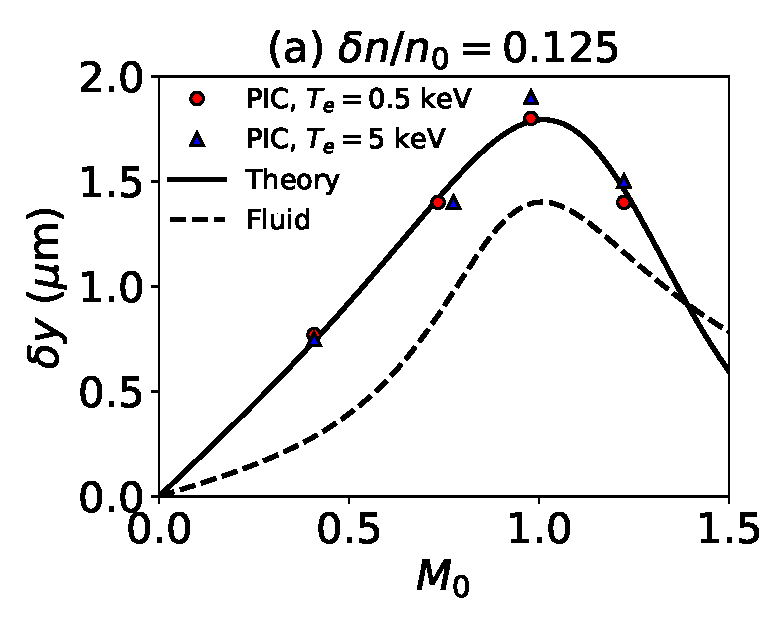
\includegraphics[scale=0.49]{th_PIC_dnsn1s8a.eps} \\
\includegraphics[scale=0.49]{th_PIC_dnsn0p2b.eps}
\end{tabular}
\caption{ \label{fig:comthpic}  
Comparison between the theoretical predictions of the laser centro\"id displacement $\langle y \rangle_y$ from Eq. \eqref{eq:dy} with $n_e/n_c=0.1$, $L_x=100 \,\mu m$ and $\delta n_0/n_0=0.0625$ (a) and $\delta n_0/n_0=0.2$ (b) as black solid line. Numerical results (see text) obtained with $T_e=500$ eV (circles) and $T_e=5$ keV  (triangles) are superimposed. The fluid theory obtained from the numerical integration of Eqs. \eqref{eq:dthetarose26}-\eqref{eq:frose26} \cite{POP_Rose_96} is illustrated by the black dashed lines.
}
\end{figure}

For sake of completeness, a larger value of $\delta n_0/n_0=0.2$, marginally in the small density perturbations limit ($\delta n_0/n_0 \ll 1$) of Eq.  \eqref{eq:drakef} has also been addressed in Fig. \ref{fig:comthpic}(b).
In this case, the estimation of our  numerical results (as circles and triangles) that are underestimated  by our linear theoretical predictions (solid line), requires a nonlinear correction, as the one suggested by  Ref.
\cite[]{PRL_Casanova_85,PFB_Rozmus_1992}.

Although no Brillouin back scattering are observed in our simulations, backward (BSRS) and forward (FSRS) stimulated Raman scattering modes are captured for the cases $T_e=500$ eV ($T_e=5$ keV respectively). 
In our simulations, FSRS is observed at the beginning only, vanishing as soon as the pump wave starts to be deflected off its original course, after a few picoseconds. As seen in the resulting intensity profiles, the superposition of the pump and diffused waves results in an increase of the opening angle of the laser beam that rapidly  disappear.
Regarding FSRS for the case $T_e=500$ eV, a backscattering of less than \textcolor{red}{ 5\%} is observed in our simulations, hence, we may neglect the pump depletion that can affect the ponderomotive density fluctuations [see Eq. \eqref{eq:drake}] and thus the beam bending predictions.
\textcolor{red}{ 
The saturations of Raman scattering is known to produce a low density hot electron population of energy given by $\sim m_e v_\phi^2 $ with $v_\phi =$ resulting to a hot electron temperature 
$T_{eh}\sim 40$ keV and $\sim 200$ keV } in fair accordance with the PIC simulations results.  The hot electron density in our simulations verifies 
\textcolor{red}{ $n_{eh}\sim [0.001-0.01]n_e$  } and remain dilute throughout our simulations. 

It is interesting to look at the influence of such a population on the beam bending rates. For the superpostion of the two Maxwellian electron populations ($e$ and $eh$-subscript) the kinetic factor of Eq. \eqref{eq:drakef} becomes 
\begin{align}
 \alpha_ \mathrm{kin}    =\frac{1}{2} \frac{-\mathcal{Z}'( \xi_i) [\mathcal{Z}'( \xi_e)  +\frac{n_{eh}T_e}{n_eT_{eh}}\mathcal{Z}'( \xi_{eh})] }{  \mathcal{Z}'( \xi_i) +[\mathcal{Z}'( \xi_e)  +\frac{n_{eh}T_e}{n_eT_{eh}}\mathcal{Z}'( \xi_{eh})]\frac{ T_i }{  ZT_e} } \, . \label{eq:drakefeh} 
\end{align}
For all our simulation $n_{eh}T_e/ (n_eT_{eh}) \ll 1$ which seems to indicate that the Raman hot electron population may not affect the beam bending physics of interest here. 

\subsection{Corrected ponderomotive potential and transient regime} \label{sec:transient}
\begin{figure}
\begin{tabular}{c}
\includegraphics[scale=0.49]{fig3a.png} \\
\includegraphics[scale=0.49]{fig3b.png} \\
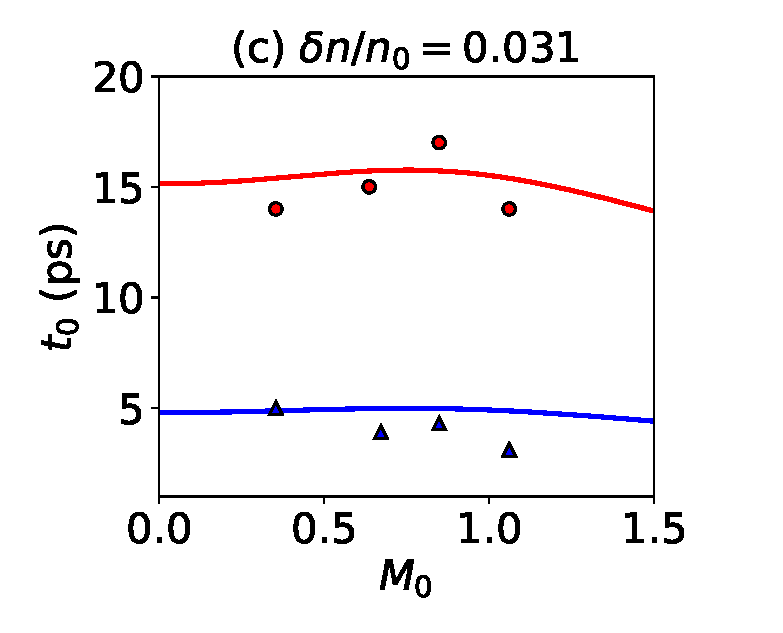
\includegraphics[scale=0.49]{th_PIC_t0.eps}
\end{tabular}
\caption{ \label{fig:transient}  
(a) Intensity lineout at the exit plane of the simulation,  $x = 128 \,\rm\mu m$, as  a function of time for the case $I_0 = 3\times 10^{14} \,\rm W.cm^2$, $T_e=500$ eV, $T_i=3$ keV, and $ v_d=0.9c_s$. The maximum of the intensity is illustrated by a thin red line while the  theoretical predictions of Eq. \eqref{eq:tr} is represented by the thick red line.
(b) Comparison between $t_0$ from Eq. \eqref{eq:t0} and the time for which the intensity maximum displacement extracted from the simulation fulfills $\delta y = (1-\exp(-1))\delta y ^{\infty}$, \emph{i.e.} reaches   63\% of its asymptotic value.  The numerical results corresponds $\delta n/n=0.0625$  with   $T_e=500$ eV (red circles) and $T_e=5$ keV  (blue triangles).}
\end{figure}
Regarding the transient regime, the proper analytical modeling requires to account for the evolution of the  kinetic Landau damping of a growing driven acoustic wave; this formidable task, as done in Ref. \cite[]{POP_Benisti_2015}  for   electron waves, is out of the scope of this manuscript. 

Following Ref. \cite[]{POP_Debayle_2018}, we will use the fluid framework to model analytically  the beam-bending transient regime. In order to make sure that the ponderomotive force applied to the hydrodynamic equations leads to the correct asymptotic regime, the kinetic density fluctuations of Eq. \eqref{eq:drakef}  will be identify to the solution of Eq. \eqref{eq:hydro3b}, which, for a Landau ion acoustic wave damping rate that verifies $\nu=\gamma_0c_s \vert k_y\vert$, reads 
\begin{equation}
\left(\frac{\delta n}{n}\right)_\mathrm{hydro} =\frac{-\Phi}{1-M_0^2 -2i M_0 \frac{nu}{k_y c_s}} \, .
\end{equation} 
we thus deduce 
\begin{equation}
\left(\frac{\delta n}{n}\right)_\mathrm{Kin} =\left(1-M_0^2 -2iM_0\frac{\nu}{k_y c_s} \right)  \alpha_\mathrm{kin}
%\left(\frac{k_y v_d}{\vert k \vert }\right)
\left(\frac{\delta n}{n}\right)_\mathrm{hydro}\, .
\end{equation} 
For $M_0 =0$, $\alpha_\mathrm{kin}=1$, so that $(\delta n/n)_\mathrm{Kin} = (\delta n/n)_\mathrm{hydro}$.
The corrected hydrodynamical equation in its linearized form becomes 
\begin{align}
 \{ (c_s^2-v_d^2)\partial_y^2 -\partial_t \partial_t\}    \frac{  \delta n }{n_0} - 2 v_d \partial_y  \partial_t \frac{  \delta n }{n_0}   \nonumber \\
-2\nu  (\partial_t + v_d  \cdot \partial_y) \frac{  \delta n }{n_0}   = - c_s^2\partial_y^2 \hat{\Phi} \, , \label{eq:hydrof2} \\
 \hat{\Phi}_k  =\left(1-M_0^2 -2iM_0\frac{\nu}{k_y c_s}\right)    \alpha_\mathrm{kin}\left(\frac{k_y v_d}{\vert k_y \vert }\right)\Phi_k  \, .\label{eq:hydrof3} 
\end{align}
The value of $\hat{\Phi}$ is related to ponderomotive potential, $\hat{\Phi}$, through a complex scalar that introduces a phase shift between the density minimum and the intensity maximum. The right hand side of Eq. \eqref{eq:hydrof2} has been implemented in the hydrodynamic  code HERA  by computing Eq. \eqref{eq:hydrof3} after a Fourier transform in the direction transverse to the main laser axis. Before applying the inverse Fourier transform back to the real space, one can also include the thermal corrections of Ref. \cite[]{Bychenkov_2000} although not used in this study.
\textcolor{red}{Finally, as will be shown subsequently, the value of $\nu$  is critical for describing  the transient regime. Hence, Landau damping has been implemented in HERA, as described in Ref. \cite[]{harmony}.}

In order to  model the transient regime of beam bending and solve Eqs. \eqref{eq:hydrof2}-\eqref{eq:hydrof3}, we could use the analytical  solution of Ref. \cite[]{POP_Huller_2020} where the full spatiotemporal linear response of  a flowing plasma to a ponderomotive pressure is derived in the hydrodynamic framework. However, the parameters of interest here ($ZT_e/T_i\sim 1$) are out of reach of these equations that were derived assuming $\nu\sigma/c_s\ll 1$. Indeed, evaluating $\left \langle\partial_y  \left( \delta n  \right)  \right  \rangle_y  $ with Eq. (16) of Ref. \cite[]{POP_Huller_2020}  gives,  for our parameters ($ZT_e/T_i\sim 1$),  a temporal evolution that unphysically overshoot its asymptotic limit by a factor $\gtrsim 2$ [see Fig. \ref{fig:transient}(a)]. 

Instead, we note that Eqs \eqref{eq:hydrof2}-\eqref{eq:hydrof3}, after a transverse spatial Fourier transform and  written in the plasma rest frame (for $M_0=v_d=0$),  coincide with Eq.  (10)  of  Ref. \cite[]{POP_Debayle_2018} that has been solved exactly [Eq. (12)]. 
Unlike in Ref. \cite[]{POP_Debayle_2018} where  the free wave characteristics,  $\omega$, $k_y$ and $\nu$ are unambiguous, the ponderomotive force drives in our case, density fluctuations with a significant spectral width [$\sim  g(k_y)= \exp(-k_y^2\sigma^2 /8)$]. 
We will estimate the relevant free wave damping rate, $\nu=\gamma_0 c_s \vert k_y \vert$ by using the averaged of Eq. \eqref{eq:kmoy},
\begin{align}
 \langle \vert k_y\vert  \rangle_{k_y}\equiv \frac{\int dk\vert k\vert  e^{-k^2\sigma^2 /8} }{\int dk e^{-k^2\sigma^2 /8}} & = \frac{2}{\sigma \sqrt{\pi}}\, , \\
 \langle \nu \rangle_{k_y} & = \frac{2\gamma_0 c_s}{\sigma \sqrt{\pi}}\, , \\
\omega  & = \frac{2c_s}{\sigma \sqrt{\pi}}\, .
\end{align}

Hence, the temporal evolution of the displacement and deflection angle can be related to their asymptotic values through
\begin{align}
    \Delta y (t) = f(t)\Delta y^\infty \, , \label{eq:dyt} \\
    \Delta \theta (t) = f(t)\Delta \theta^\infty \, , \label{eq:dtht}
\end{align}
with, for a laser intensity independent of time and $\omega^2 > \langle \nu \rangle_{k_y} ^2$,
\begin{align}
 f(t)  &= 1 -e^{- \langle \nu \rangle_{k_y}  t}[\cos(at)+ \langle \nu \rangle_{k_y}  \sin(at)] \cos(\omega t)\nonumber \\
 &-\frac{\omega}{a} e^{- \langle \nu \rangle_{k_y}  t}  \sin(at) \sin(\omega t)\, ,\label{eq:ft}\\
 a &= \sqrt{\omega^2 - \langle \nu \rangle_{k_y}^2} \label{eq:fta}\, .
\end{align}
Hence, the bending angle of a pulse reaches its asymptotic limit in a  few a free acoustic Landau damping times.
The temporal evolution of the pulse intensity profile is illustrated in Figs. \ref{fig:transient}(a,b) for the case $\delta n/n=0.031$, $T_e=500$ eV and $T_e=5$ keV. 
The location of  the intensity maximum  as a thin red line presents a slow rise  until \textcolor{red}{$20$ ps  (a) [$7$ ps  (b)]
before reaching the asymptotic limit of $ \sim1.8 \,\rm \mu m$ (a) [$ \sim1.2 \,\rm \mu m$  ps  (b)] and agrees correctly with the analytical predictions of Eq. \eqref{eq:dyt}-\eqref{eq:fta}. 
}
The time, $t_0$, for which the intensity  displacement reaches $f(t=t_0)=1-\exp(-1)\simeq 63\%$ of its asymptotic value can be extracted from the theory and the simulations and compared. Figure \ref{fig:transient}(c) presents a fair agreement between the theoretical values  of  $t_0$ [obtained by solving numerically $f(t)=e^{-1}$, Eq. \eqref{eq:ft}] and the one extracted from the PIC simulations. Thus, the beam bending transient regime may be modeled through Eqs. \eqref{eq:dyt} and \eqref{eq:dtht}, for $M_0<1.5$. 

\section{Modified ray tracing scheme}
So as to model the propagation of a RPP-beam in a flowing plasma, we propose here the reconstruction of the laser intensity pattern near the focal plane in an hydrodynamic code using a Monte-Carlo scheme to account for the influence of the local intensity maximum, \emph{i.e.} the speckles, on the beam bending physics.

\subsection{RPP-beam spatial spectrum}
The RPP smoothing technique applied to a coherent light wave results in the broadening of the spatial electromagnetic spectrum transversely to the laser propagation direction. 
The simplest model of the field profile at the focal plane, used in \cite[]{POF_Schmitt_88,POF_Rose_93}, consists in a uniformly distributed field in the transverse Fourier space around the light wave number. At best focus, $x=x_\mathrm{foc}$, the electric field reads
\begin{align}
    E_\mathrm{RPP}(y,t) =E_0 e^{i (k_0 x -\omega_0 t ) }   \sum_{k_y} \mathrm{H}( k_\mathrm{max} - \vert k_y \vert )e^{i k_y y +i\phi_{k_y}  }  \, , \label{eq:efoc}
\end{align}
where the phases $\phi_{k_y}$  are independent random variables taking the values $0$ or $\pi$ with equal probability. $\mathrm{H}$ and  $k_\mathrm{max}$ are the unity step function and a cutoff wave vector, respectively. The effective focal number of the speckle, $f$, can be related to  $k_\mathrm{max}$ through  $k_\mathrm{max}=k_0/2f$ assuming $f\gg 1$.
In the following, the sum in Eq. \eqref{eq:efoc} can be recast using $k_\perp =  n k_\mathrm{max}/N$ with $n\in[\![-N,N]\!]$. In this work, the number of diffracting elements is fixed to $2N=100$.
%Regarding the intensity ....
Note that the ratio $k_y/k_0$ can be seen as the angle of propagation of the beamlet in the small angle limit ($k_y/k_0\ll1$). Hence,   the local opening angle of the beamlet is $2k_\mathrm{max}/k_0 = 1/f$ in vacuum.
%
%Likewise, .... 

Let introduce the spatial, $\hat{g}(y)$, and temporal, $h(t)$, envelopes at best focus. Within the para-axial approximation, the boundary condition at $x=x_\mathrm{BC}$ can be found by multiplying Eq. \eqref{eq:efoc} by $h(t)*\hat{g}(y)$  and  apply the well-known Fresnel integral:
\begin{align}
    E(x_\mathrm{BC},y,t) =&h(t)e^{i\omega t}\times  \nonumber \\
    &\mathrm{FT}^{-1}_y \left\{ e^{i \frac{k^2 (x_\mathrm{foc}-x_\mathrm{BC}) }{2k_0}} 
   \mathrm{FT}_k \left[ \hat{g}(y)E_\mathrm{RPP} \right]  \right\}  \, , \label{eq:ebc}
\end{align}
where $FT_k$ and $FT^{-1}_y$ are the direct and inverse Fourier transform. 

\subsection{Intensity profile in vacuum and beam-bending model}
For sake of completeness, the main speckle spatial properties in vacuum are recalled in the following, according to the analytical derivations of Ref. \cite{Garnier_1999}. 
The hot-spot number per volume unit in vacuum, $\mathcal{N}^\mathrm{vac} $, depends on the ratio between the maximum hot spot intensity $ I_{s,0}$ and the averaged intensity $\langle I \rangle$. It follows 
\begin{align}
\mathcal{N}^\mathrm{vac} =\prod_{d=1}^{D}   \frac{1}{\lambda^\mathrm{vac}_d}   \, ,\label{eq:ncal} 
\end{align}
which involves a product on the dimensions ($d$-subscript, with $D$ the dimension number) and where $\lambda_d$ is the averaged distance between each hot spots in the direction $d$.
For $D =2$, or $3$, it reads:
\begin{align}
&\lambda^\mathrm{vac}_\parallel\left( \frac{I_{s}}{ \langle I \rangle }   \right)=\frac{1}{g_D^{1/D} }  z_c  \, ,\label{eq:ldx} \\
&\lambda^\mathrm{vac}_\perp \left( \frac{ I_{s}}{ \langle I \rangle }   \right)=\frac{1}{g_D^{1/D} }  \rho_c  \, ,\label{eq:ldy} \\
&g_{2} = \frac{\pi}{ 3\sqrt{15} }\left[ \left( \frac{1}{ 2 } +\frac{\pi}{ 4 }\right)\frac{I_{s}}{ \langle I \rangle }  +\frac{1}{ 2 } \right] e^{- \dfrac{ I_{s}}{ \langle I \rangle }  }  \, ,\label{eq:f2} \\
&g_{3} = \frac{\pi^{3/2}\sqrt{5}}{ 27 }\left[ \left( \frac{ I_{s}}{ \langle I \rangle }   \right)^{3/2} -\frac{3}{ 10 } \left( \frac{ I_{s}}{ \langle I \rangle }   \right)^{1/2}  \right] e^{- \dfrac{ I_{s}}{ \langle I \rangle }  } \, . \label{eq:f3} 
\end{align}

 For a given RPP beam, the ray tracing scheme resolves the Eikonal equation to obtain the ray paths in the simulation box.
Restricting the following to a two dimensional case for a beam propagating along the $x$ direction (so that $x\equiv \parallel$ and $y\equiv \perp$), the spatial distribution of the speckle population may be reconstructed by a Monte Carlo scheme, using  $\lambda^\mathrm{vac}_\parallel$ and $\lambda^\mathrm{vac}_\perp$ as correlation length.
By binning the hot spots population regarding their intensity amplitude, $I_{s}$, we may compute the inter-speckle distances 
associated with each intensity bundle.
As the correlation lengths are increasing function of the speckle intensity, the bundles with the largest intensity will corresponds to the rarest speckles in the beam and to the largest beam bending angle [see Eq. \eqref{eq:dthf}].
%\textcolor{red}{Moreover, the use of the Gaussian calculations of Sec. \ref{sec:gauss} for modeling the speckle-scale beam bending implies that  each intensity maximum behaves independently from each other, which along Ref. \cite[]{Huller_1997}, is fulfilled for $I_{s,0}\gtrsim 3-5 \langle I \rangle $.}
\textcolor{red}{
We will thus subsequently  bin the speckles intensity according to the local intensity (calculated in the mesh) starting from $I_{s,\mathrm{min}} =  2 \langle I \rangle$ up to  $I_{s,\mathrm{max}} =  2n_c v_gT_e/3$, which corresponds to $\delta n/n =1/3$, 
\emph{i.e.} assumed to be the marginal  validity regime of the linearized plasma response used to derive Eq. \eqref{eq:drake}. 
}
Note that the speckles of  intensity larger than  $ 2n_c v_gT_e/3$ are considered as out of reach by the present model due to their nonlinear behavior. %\textcolor{red}{Likewise, the speckles of  intensity lower than $5\langle I \rangle$, may collectively amplify an acoustic perturbation such as the one expected for forward stimulated Brillouin scattering or other plasma smoothing effects \cite{POP_Grech_2006,PRL_Grech_2009}}.

We now introduce the distances crossed by the ray in a given hydrodynamic mesh $\delta x$ and $\delta y$. 
During the Eikonal resolution, each time a ray exits an hydrodynamic mesh and for each intensity bundle,  two random numbers are shot  on the Poisson distribution with  the parameters $\delta x/\lambda^\mathrm{ray}_\parallel$ and $\delta y /\lambda^\mathrm{ray}_\perp$, where $\lambda^\mathrm{ray}_\parallel$ and $\lambda^\mathrm{ray}_\perp$ are the speckle correlation lengths used for the ray tracing scheme that will be related to $\lambda^\mathrm{vac}_\parallel$ and $\lambda^\mathrm{vac}_\perp$ subsequently.
Hence, each time a ray exits  a mesh a total of $2N_\mathrm{bundle}$ can be shot. 
This yields the number of speckles crossed by the ray in the mesh. As the ray exits the mesh and if at least one speckle has been crossed, a rotation  of the ray direction of an angle given  Eqs. \eqref{eq:dthf} and \eqref{eq:dtht}  is applied once, at the mesh exit. Moreover, only one deflection per ray is applied thus avoiding nonphysical cascade. Note that we do not modify the trajectory of the ray inside the mesh and that  Eq. \eqref{eq:dyt} include the transient regime of importance over the first few 10 picoseconds of the bending that could be ignored by setting $f(t)=1$. Choice has been made in this study to use Eqs. \eqref{eq:ft}-\eqref{eq:fta} calculated on the local plasma parameters with $t$ as the simulation time. 

Our full PIC  simulations show that essentially most of the pulse power, $P^\mathrm{speckle}= I_s\sigma \sqrt{\pi}$ is deflected.
Hence,  the number of rays that needs to be 
rotated per speckle in order to account for the write quantity of deflected power  can be related to the ratio  $P^\mathrm{speckle}/P^\mathrm{ray}$ where $P^\mathrm{ray}$ is the power carried by one ray in vacuum. 
%%%%%%%%%%%
It follows
a correction to the number of speckle in vacuum that must be applied for each  intensity bundle.
%%%%%%%%%%%
The corrected speckle number in our ray tracing scheme thus reads $\mathcal{N}^\mathrm{ray}=  \mathcal{N}^\mathrm{vac}P^\mathrm{speckle}/P^\mathrm{ray} $, which gives with Eq. \eqref{eq:ncal}
\begin{align}
\lambda^\mathrm{ray}_\parallel & = \left( \frac{P^\mathrm{ray}}{ I_s\sigma \sqrt{\pi} } \right)^{1/D} \lambda^\mathrm{vac}_\parallel \, ,\label{eq:ldxr} \\
\lambda^\mathrm{ray}_\perp   & = \left( \frac{P^\mathrm{ray}}{ I_s\sigma \sqrt{\pi} } \right)^{1/D}  \lambda^\mathrm{vac}\, ,\label{eq:ldyr}  
\end{align}
As one increases the number of rays that resolves a given RPP pulse, thus decreasing $P^\mathrm{ray}$, more and more rays needs to be deflected for accounting for the physical amount of bending.

The above model has been implemented in a new  ray  tracing module of the hydrodynamical code HERA \cite[]{}.
For solving the ray trajectory, we split the rectangular meshes in four triangles using their diagonals.  In each triangle, the density profile is assumed to be planar allowing to have a continuous density profile in all the simulation domain. 
Hence, solving the Eikonal equation in each triangle allows to break the ray trajectory in a row of parabolas ideal for fast computing. 
Summing the contribution of each rays that pass through a given mesh following Ref. \cite[]{POP_Debayle_2019}, one obtains the local averaged intensity, $ \langle I\rangle$, used in the speckle modeling [in Eqs. \eqref{eq:ldx}-\eqref{eq:ldyr}].
So has to mimic the averaged intensity profile at and off best focus, we define a lens position, hereafter at $x_\mathrm{lens}=-10$ m from which rays are shot \cite[]{Lefebvre_2018}. 
The rays departure $y$-positions  on the lens are chosen randomly, and their initial direction points toward a randomly distributed  position at the focal plane (at $x=x_\mathrm{foc}$) which ascertain the power carried by the ray so as to fulfill the required intensity profile at best focus [given by $g(y)$]. 
Finally, the rays are propagated  in vacuum from the lens to the left boundary condition  of the simulation (at $x=x_\mathrm{BC}$).
In order to avoid statistical bias, the position and directions of the rays are shot at beginning of each time steps. 
Note that this procedure locally gives a  finite   transverse opening angle to the ray distribution, thus avoiding unphysical filamentation  arising for perfectly parallel rays. 

\subsection{Comparison between PIC,  corrected paraxial hydrodynamics and ray tracing simulations}
\begin{figure*}
\begin{tabular}{ccc}
\includegraphics[scale=0.39]{Figure/I_Smilei24ps_te500eV_C6p.png}
&\includegraphics[scale=0.39]{Figure/I_HERA24ps_te500eV_C6p.png}
&\includegraphics[scale=0.39]{Figure/I_HERA24ps_te500eV_C6p.png}\\
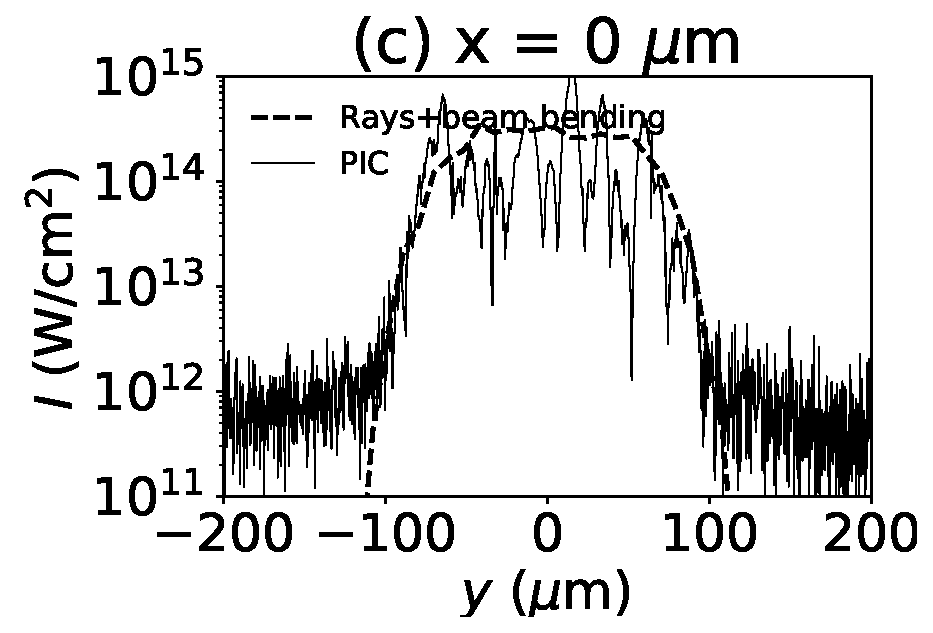
\includegraphics[scale=0.39]{Figure/Icut0_te500_C6p.eps}
&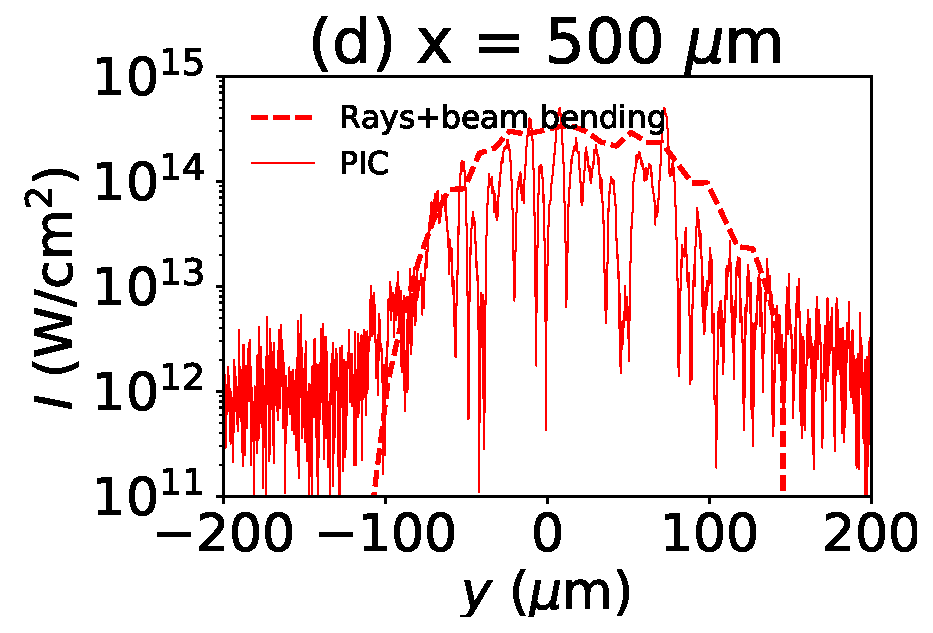
\includegraphics[scale=0.39]{Figure/Icut500_te500_C6p.eps}
&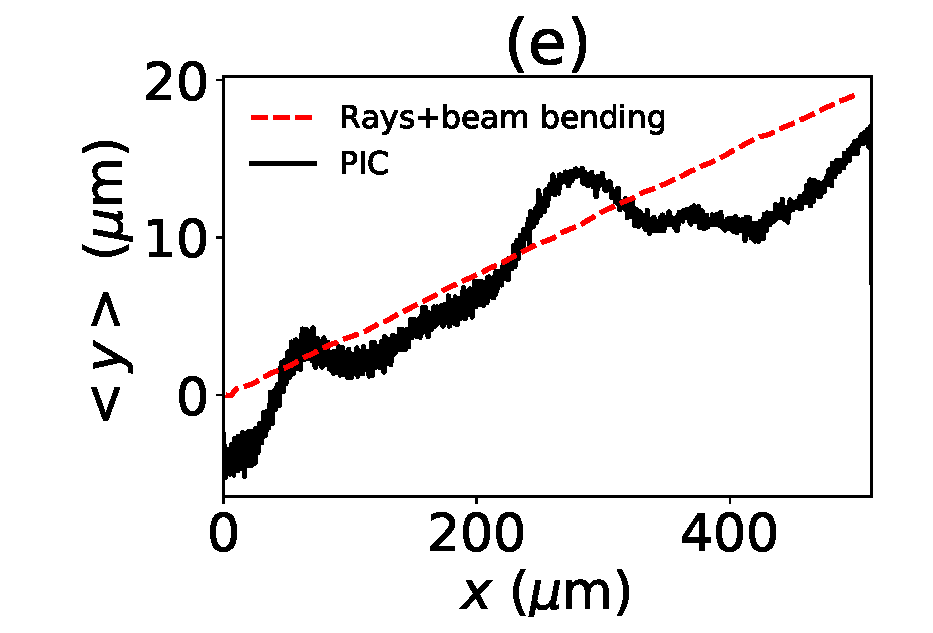
\includegraphics[scale=0.39]{Figure/ymoy_te500_C6p.eps}
\end{tabular}
\caption{ \label{fig:comthpicrpp} 
 Intensity in logscale at $t = 24$ ps of an RPP beam injected according to Eq. \eqref{eq:ebc} on the left boundary from a full PIC simulation (a), from hydrodynamics (HERA) with a paraxial propagation of the RPP beam including the correction of Eq. \eqref{eq:hydrof3} (b) and from the modified ray tracing model (c).  Lineout at $x=0$ (d) and $x=500 \, \rm \mu m$ (e) of   panel (a), (b) and (c). 
 (f) Centro\"id position (\emph{i.e.} the transverse position averaged over the intensity) from the PIC results (black solid line), from paraxial hydrodynamics (blue dashed) and  from the ray tracing scheme (red dashed line). The parameters of the C$^{6+}$ plasma are $n_e=0.1n_c$, $T_e=500$ eV, $T_i=3$ keV and $v_d=0.84 c_s$. }
\end{figure*}
\begin{figure*}
\begin{tabular}{ccc}
\includegraphics[scale=0.39]{Figure/I_Smilei18ps_te1keV_Ti1keV_.png}
&\includegraphics[scale=0.39]{Figure/I_HERA18ps_te1keV_Ti1keV_.png}
&\includegraphics[scale=0.39]{Figure/I_HERA18ps_te1keV_Ti1keV_.png}\\
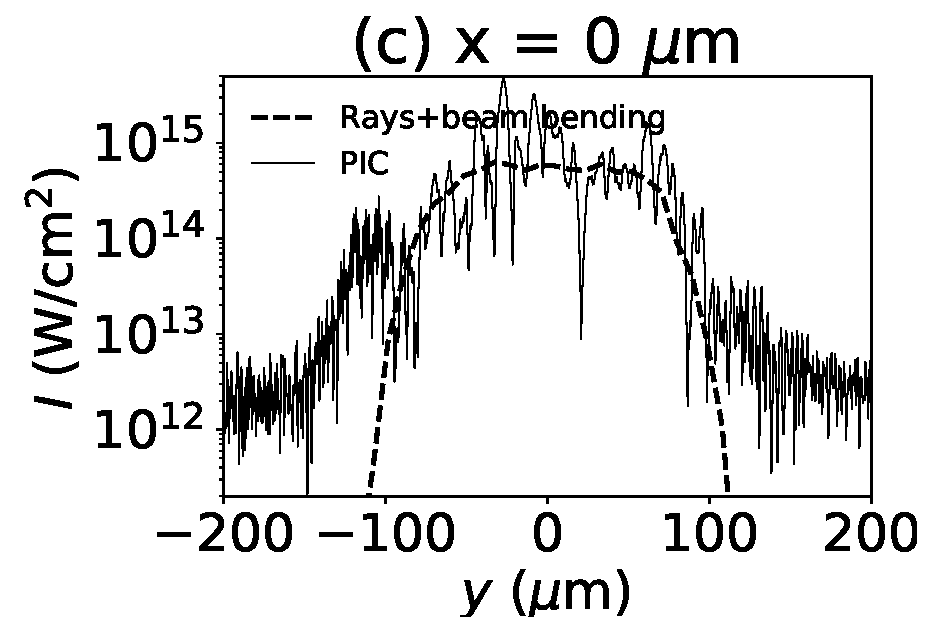
\includegraphics[scale=0.39]{Figure/Icut0_te1keV_Ti1keV_.eps}
&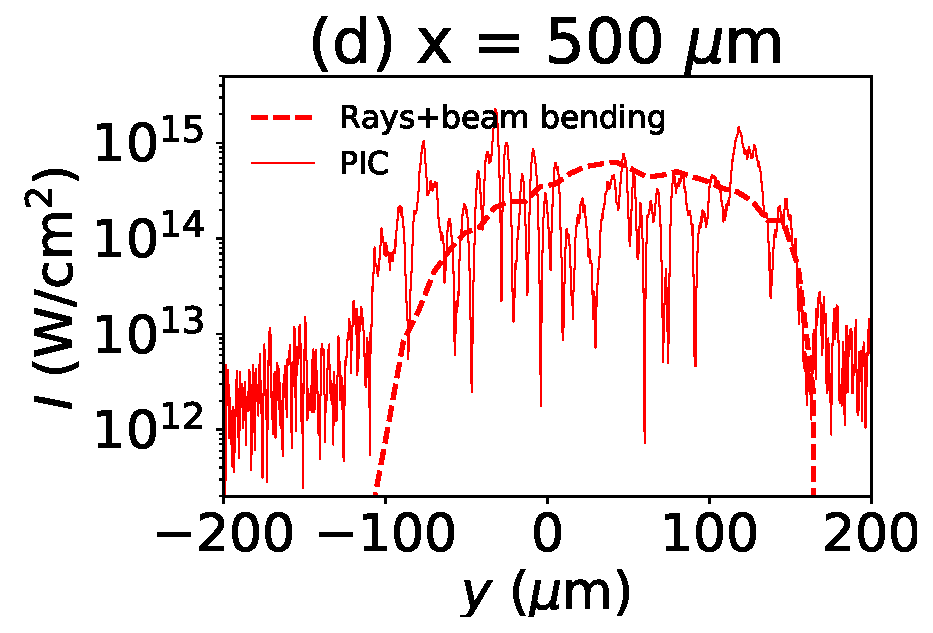
\includegraphics[scale=0.39]{Figure/Icut500_te1keV_Ti1keV_.eps}
&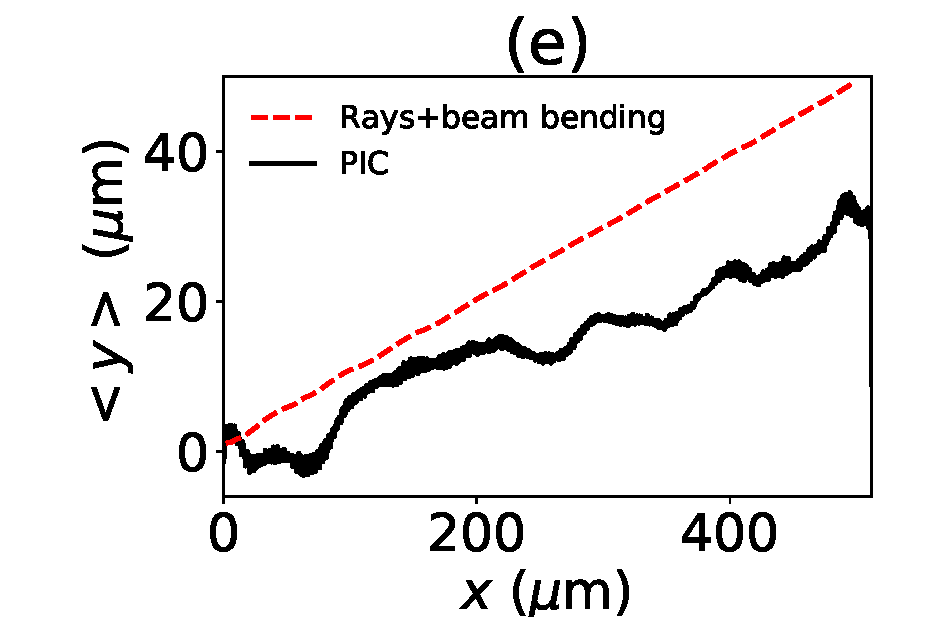
\includegraphics[scale=0.39]{Figure/ymoy_te1keV_Ti1keV_.eps}
\end{tabular}
\caption{ \label{fig:comthpicrpp2} 
Similar figures than in Fig. \ref{fig:comthpicrpp} for a H$^{+}$-plasma with $n_e=0.1n_c$, $T_e=1$ keV, $T_i=1$ keV, and $v_d=0.84 c_s$ at time $t= 18$ ps.  }
\end{figure*}
\begin{figure*}
\begin{tabular}{ccc}
\includegraphics[scale=0.39]{Figure/I_Smilei20ps_te1keV_Ti300eV_.png}
&\includegraphics[scale=0.39]{Figure/I_HERA20ps_te1keV_Ti300eV_.png}
&\includegraphics[scale=0.39]{Figure/I_HERA20ps_te1keV_Ti300eV_.png}\\
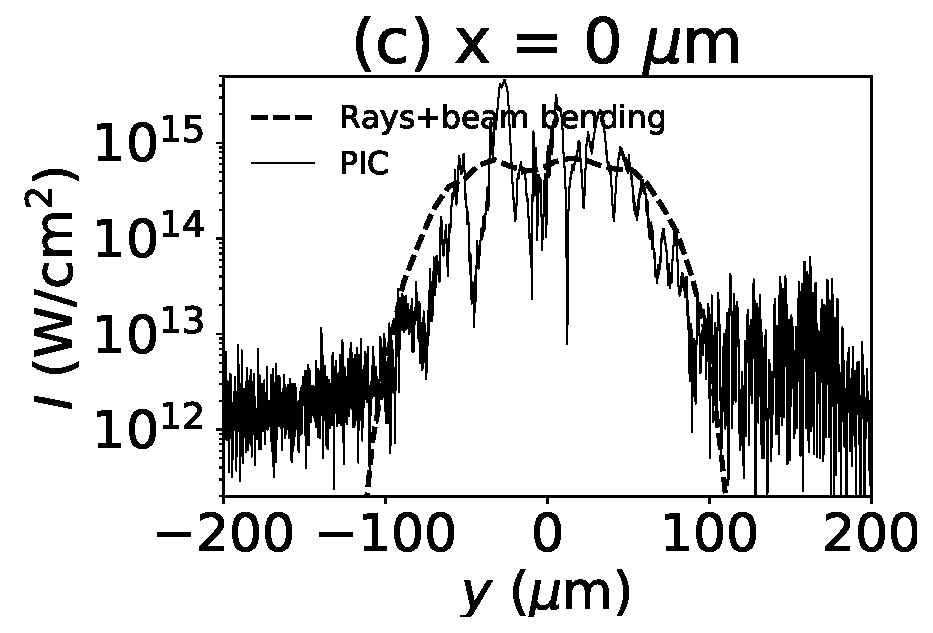
\includegraphics[scale=0.39]{Figure/Icut0_te1keV_Ti300eV_.eps}
&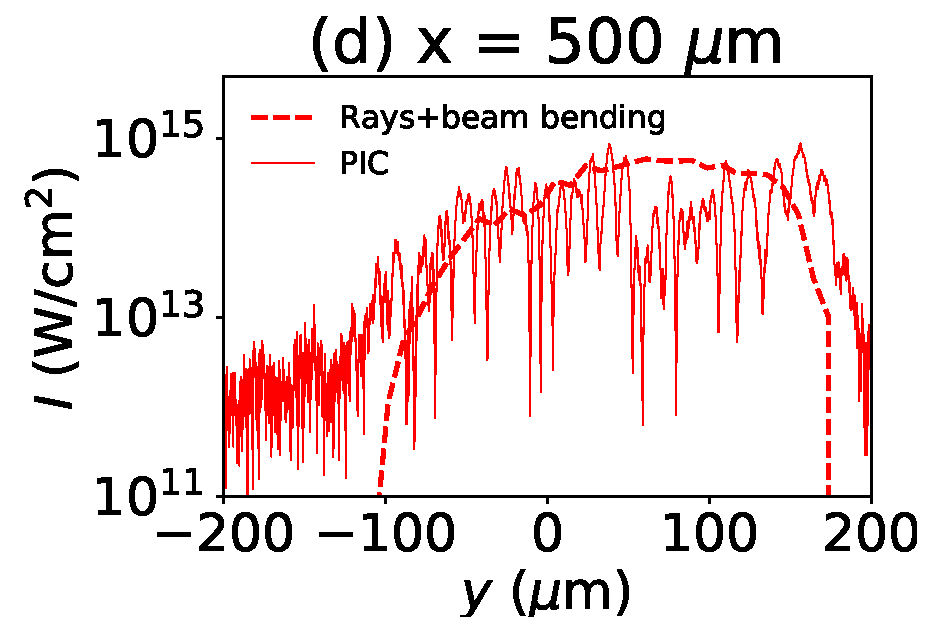
\includegraphics[scale=0.39]{Figure/Icut500_te1keV_Ti300eV_.eps}
&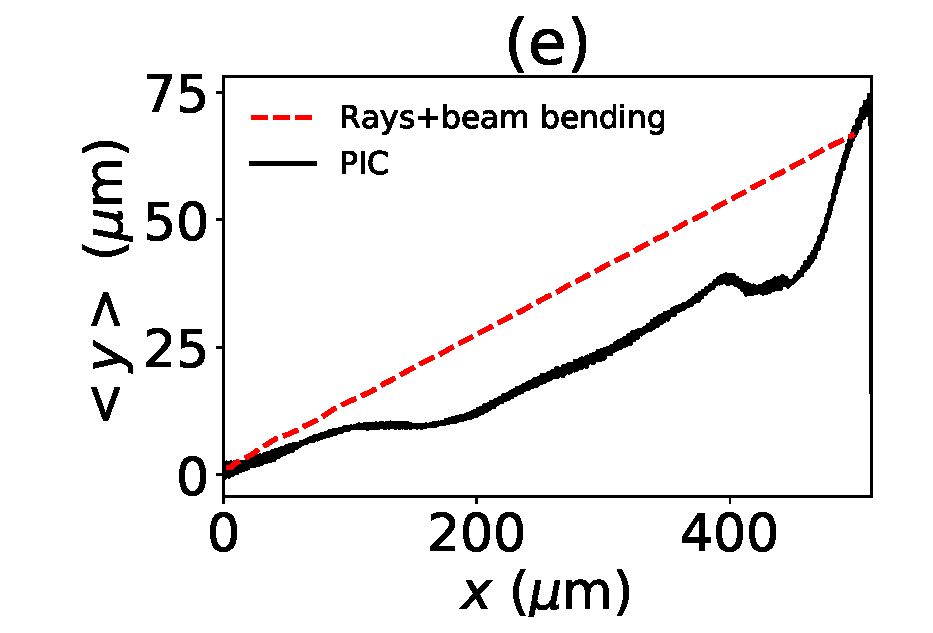
\includegraphics[scale=0.39]{Figure/ymoy_te1keV_Ti300eV_.eps}
\end{tabular}
\caption{ \label{fig:comthpicrpp3} 
Similar figures than in Fig. \ref{fig:comthpicrpp} for a  H$^{+}$-plasma with $n_e=0.1n_c$, $T_e=1$ keV, $T_i=300$ eV and $v_d=0.84 c_s$, at time $t = 20$ ps.
 \textcolor{red}{Mettre comparaison bin number et resolution}}
\end{figure*}

A quantitative comparison may now be carried between the  
exact solution obtained from large scale PIC simulations (with Smilei) and two types of  hydrodynamic simulations.
The first kind (HERA-ray) uses   HERA   with the modified ray tracing scheme (with large mesh size) and the second,  (HERA-parax) a paraxial solver (resolving the laser wavelength) for the RPP beam combined with the corrected ponderomove force introduced in Eqs. \eqref{eq:hydrof2}-\eqref{eq:hydrof3}. 

For all simulations codes, a 2D domain of size $L_x \times L_y = 512 \times 512\, \rm \mu$m$^2$ with the left boundary condition located at $x_\mathrm{BC}=0$ will be used. 
A RPP-beam (using Eqs. \eqref{eq:efoc} and  \eqref{eq:ebc}) or a ray tracing beam propagating in the $x$ direction were injected from the left boundary.
The focal spot is located at the center of the simulation domain, $x_\mathrm{foc}=256\, \rm \mu m$ with a speckle effective focal number of $f = 6.5$, a temporal
and spatial envelope following
\begin{align}
    \hat{g}(y) &= \exp(-\vert y\vert ^o/2\sigma_g^o)  \,  \\
    h(t) &= \mathrm{min}(t/\tau_h,1) \,
\end{align}
with a $\tau_h=1\, \rm ps$,  $o=5$ and $\sigma_g = 70\,\rm \mu m$. 
For sake of simplicity and comparison purposes, the bremsstrahlung energy deposition is neglected in HERA-ray and HERA-parax and does not occur in the collisionless PIC simulations.  Moreover perfect gaz is assumed in the hydrodynamics simulations.
As in Sec. \ref{sec:gauss}, all simulations in this study have been performed with $T_i \sim ZT_e$ in order to maximize the free-mode acoustic damping rate and therefore reduce as much as possible the stimulated Brillouin backward scattering. Moreover,  a total electron density of $n_e =0.1n_c $ is used  and a $y$-aligned drift velocity, $v_y=v_d$, is imposed on both the electron and ion populations.


Regarding the PIC simulations,  fully periodic boundary  conditions in the $y$ boundaries are applied for both fields and particles. Silver-M\"uller absorbent for the field and \textcolor{red}{absorbent} for the particles are used in the $x$ boundaries.  
A fourth order interpolation scheme is used with 36 particles per mesh per species, 21 points per laser wavelength and 14 points per laser temporal period. The plasma density is constant everywhere except on 12 microns close to both $x$ boundaries so that the effective plasma length is $0.488$  mm.

Regarding HERA-parax, use has been made of $dx =\lambda_0$, $dy = 0.125\lambda_0$ and $dt=10^{-13}$ s, \textcolor{red}{BC !}. 

In all two dimensional HERA-ray simulations shown in this study, the Cartesian grid has a mesh size of $dx=3.91\lambda_0$, $dy=9.37\lambda_0$ and $dt=5\times 10^{-13}$ s , much larger than the laser wavelength. The ray schemes use $10^4$ rays with regular speckle intensity bundles of width $dI/\langle I \rangle=0.1$ ranging from $I_\mathrm{max}/\langle I \rangle=2$ to $I_\mathrm{min}/\langle I \rangle=10$. \textcolor{red}{BC !}. 

The beam bending rate has been validated with three sets of parameters, namely a C$^{6+}$ plasma with $(T_e, T_i )= (500\, $eV$, 3\, $keV$)$ with an averaged laser intensity of $I_0 = 3\times 10^{14}\,\rm W.cm^{2}$, and a H$^{+}$ plasma  with $(T_e, T_i )= (1\, $keV$, 1 \,$keV$)$ and $(T_e, T_i )= (1\, $keV$, 300 \,$ eV$)$ with $I_0 = 6 \times 10^{14}\,\rm W.cm^{2}$.
Figs. \ref{fig:comthpicrpp}(a), \ref{fig:comthpicrpp2}(a) and \ref{fig:comthpicrpp3}(a) present the three aforementioned PIC simulations. All simulations unravel the deflection off its original course of a significant portion of the pulse energy  due to the beam bending effect.  
Very similar intensity profiles are obtained by the HERA-parax simulations illustrated in Figs. \ref{fig:comthpicrpp}(b), \ref{fig:comthpicrpp2}(b) and \ref{fig:comthpicrpp3}(b).
The ray tracing HERA-ray simulations [see Figs. \ref{fig:comthpicrpp}(c), \ref{fig:comthpicrpp2}(c) and \ref{fig:comthpicrpp3}(c)], although far less numerically constraining and neglecting the speckle-scale intensity fluctuations,   share a similar behavior than the PIC and HERA-parax simulations, \emph{i.e} more deflected light in the $y>100\,\rm\mu m$-region in the case of the H$^{+}$ than in the C$^{6+}$ plasma. 
All Smilei and HERA simulations evidence that the bending starts to affect the intensity profile for $x>200\,\rm\mu m$ for the H$^{+}$ case and  $x>300\,\rm\mu m$ for the C$^{6+}$.
\textcolor{red}{
The comparison of the intensity profiles  in Figs. \ref{fig:comthpicrpp}(c,d), \ref{fig:comthpicrpp2}(c,d) and \ref{fig:comthpicrpp3}(c,d) at $x=0$ and $500\,\rm\mu m$ illustrate the self-consistent description of the speckle scale field fluctuation in the PIC simulations (black solid lines). By contrast, the ray tracing scheme which only reproduces the averaged intensity fluctuations (red dashed lines), yield} much smoother profiles.
The laser centro\"ids, $\langle y \rangle$ [see Figs. \ref{fig:comthpicrpp}(e), \ref{fig:comthpicrpp2}(e) and \ref{fig:comthpicrpp3}(e)], measured in the PIC simulations by averaging the transverse position $y$ along the intensity transverse profile, exhibit some fluctuations. This tendency is probably due to the relatively weak number of speckle in our $\sim 70\,\rm\mu m$-focal spot, constrained by the high numerical cost of the kinetic simulations. 
The model satisfactorily captures the effect of the speckle-scale beam bending on the deflection of the averaged intensity envelope after $500\,\rm\mu m$ of propagation. 

The cases of Figs.  \ref{fig:comthpicrpp} (C$^{6+}$-plasma, $T_e=500$ eV) and Figs.  \ref{fig:comthpicrpp2} (H$^{+}$-plasma, $T_e=1$ keV)  correspond to the same values of $\delta n /n =0.031 $ and $ZT_e/T_i=1$, and therefore to the same asymptotic beam-bending rate [see Eq. \eqref{eq:dthf}]. However, Figs. \ref{fig:comthpicrpp}(a,b) present qualitatively much less deflection than in Figs. \ref{fig:comthpicrpp2}(a,b). The beam centro\"ids are shifted by $\sim 15\, \rm \mu m$ and  $\sim 40 \, \rm \mu m$ at $x=500 \, \rm \mu m$ in the C$^{6+}$  and H$^{+}$-plasma respectively [see Figs. \ref{fig:comthpicrpp}(c) and \ref{fig:comthpicrpp2}(c)].
This difference is caused by the larger temperature and therefore a shorter transient regime for the  H$^{+}$ plasma ($T_e=1$ keV, $t_0=10.5\, \rm ps$, Eq. \eqref{eq:t0}) than for the C$^{6+}$ one ($T_e=500$ eV, $t_0=21\, \rm ps$).
Hence the case of Fig. \ref{fig:comthpicrpp} is closer to the asymptotic limit and have a larger deflection angle per speckle than the case of Fig. \ref{fig:comthpicrpp2}. Such transient effects, negligible after a few tens of picoseconds of propagation of an RPP beam, is  of great importance  for understanding quantitatively the bending of temporally smoothed beams as shown subsequently.

The two sets of H$^+$-plasma simulations in   Figs. \ref{fig:comthpicrpp2} and  \ref{fig:comthpicrpp3}, 
differ only from their ions temperature, $T_i = 1000$ and $300 \, \rm eV$ respectively, giving  $\Im(\alpha_\mathrm{kin})=0.57$ and $2.59$ [see Eq. \eqref{eq:drakef}]. The driven acoustic damping rate is therefore smaller for  $T_i = 1000\, \rm eV$ than for  $300 \, \rm eV$ causing a weaker beam deflection, consistently with the line-outs at $500\,\rm \mu m$ which evidence less ledging at $y\gtrsim 100\,\rm\mu m$ and more depletion around $x\lesssim -50\,\rm\mu m$ in Fig. \ref{fig:comthpicrpp2}(c) than in  Fig. \ref{fig:comthpicrpp3}(c),  respectively. 

\textcolor{red}{Influence of the bundle number}

\section{Conclusions and prospects}

We revisited in this study the beam bending physics and shown that accounting for the accurate Landau damping of driven acoustic waves is crucial in order to  quantitatively capture the propagation of Gaussian laser pulse in a flowing plasma. 
In good agreement with dedicated PIC simulations, our bending rates analytical predictions allows the enhancement of ray tracing schemes relevant for nanoseconds and millimeter-scale hydrodynamic simulation of plasma and high-density matter  physics. We also introduced  a correction to the ponderomotive force which  accounts, in a fluid code, for the influence of kinetic driven acoustic wave damping on the density fluctuations and the resulting light propagation. 

We then demonstrated that both the ponderomotive correction and the modified ray tracing schemes correctly capture the centro\"id deviation and the amount of scattered light of an RPP beam propagating in a flowing plasma. Hence, the speckle-scale physics of crucial importance for many wave-mixing processes, may be included in coarse description of light such as  ray tracing-based schemes. 

Note that, although out of the scope of this study, the generalisation to three dimensions of the modified ray tracing scheme seems feasible. Na\"ively, in addition to deriving the main equations in three dimensions, one would only have to use the speckle abundance formulas in realistic geometry in order to accurately capture the speckle-scale bending of a RPP  pulse. 
Moreover, temporal  smoothing techniques is known to reduce the beam bending as it introduces a finite speckle coherence time of the order of a few picoseconds. The generalization of our model to three dimension and to the  modeling of SSD beams is left for future work, along with its interplay with other wave-mixing processes.

\section*{Acknowledgements}
We acknowledge fruitful discussions with the  Smilei-team, particurlarly  F. Perez, M. Grech, A. Beck and J. Derouillat.
 \textcolor{red}{We also acknowledge D. Dureau and the HERA-team for all their work on the HERA code. }
This work has been done under  the auspices of  CEA-DAM and
the simulations were performed using HPC resources at TGCC/CCRT and CEA-DAM/TERA.
\bibliography{biblio}
\end{document}
